% Please use the skeleton file you have received in the
% invitation-to-submit email, where your data are already
% filled in. Otherwise please make sure you insert your
% data according to the instructions in PoSauthmanual.pdf
\documentclass{PoS}

\newcommand{\theInvRho}{\frac{\varepsilon_{\mu^+\mu^-}}{\varepsilon_{J/\psi K^{\pm}}}}
\newcommand{\pt}{$p_{\rm{T}}$}
\newcommand{\gev}{\rm{GeV}}

\title{Beauty and charm rare decays at the LHC: prospects for Run II}

\ShortTitle{Beauty and charm rare decays}

\author{U. De Sanctis\thanks{on behalf of the ATLAS Collaboration}\\
        University of Sussex\\
        E-mail: \email{umberto.de.sanctis@cern.ch}\\}
\author{F. Dettori\thanks{on behalf of the LHCb Collaboration}\\
        CERN European Organization for Nuclear Research, Geneva, Switzerland\\
        E-mail: \email{francesco.dettori@cern.ch}\\ }
\author{\speaker{S. Fiorendi}~\thanks{on behalf of the CMS Collaboration}\\
       Universit\`a di Milano Bicocca \& INFN\\
        E-mail: \email{sara.fiorendi@cern.ch}
	}

%\author{Another Author\\
%        Affiliation\\
%        E-mail: \email{...}}

\abstract{The main results on the searches for rare decays of $B$ and $D$ mesons from ATLAS, CMS and LHCb experiments are summarised in this report. Particular attention will be given to the measurements performed by at least two of the three experiments, where common aspects and differences are highlighted. Detector improvements and perspectives of the three experiments for Run 2 ongoing data campaign are also discussed.}

\FullConference{VII Workshop italiano sulla fisica pp a LHC\\
		16-18 Maggio 2016\\
		Pisa, Italy}


\begin{document}
%\documentclass[11pt]{amsart}
%\usepackage{geometry}                % See geometry.pdf to learn the layout options. There are lots.
%\geometry{letterpaper}                   % ... or a4paper or a5paper or ... 
%%\geometry{landscape}                % Activate for for rotated page geometry
%%\usepackage[parfill]{parskip}    % Activate to begin paragraphs with an empty line rather than an indent
%\usepackage{graphicx}
%\usepackage{amssymb}
%\usepackage{epstopdf}
%\DeclareGraphicsRule{.tif}{png}{.png}{`convert #1 `dirname #1`/`basename #1 .tif`.png}
%
%\title{Brief Article}
%\author{The Author}
%%\date{}                                           % Activate to display a given date or no date
%
%\begin{document}
%\maketitle
\section{Introduction}

Rare decays proceeding via flavor changing neutral currents (FCNC) only occur at loop order and beyond in the Standard Model (SM), being forbidden at tree level.
However, in SM extensions new particles can contribute at loop or tree level, resulting in a modification of the amplitude of the process, appearance of new sources of CP violation or change in the angular distribution of final-state particles.
Therefore, information about physics beyond the SM can be gathered by searching for possible deviations from the predictions on branching fractions or angular distributions of rare decay processes.

This article reviews some of the studies on rare $b$ and $c$ decays conducted during LHC RunI by the ATLAS\cite{ATLAS}, CMS\cite{CMS} and LHCb\cite{LHCb} experiments, and outlines the perspectives for Run II measurements.\\

The LHCb detector has been specifically designed to access the physics of heavy Flavors in the forward region.
It is characterized by an excellent particle identification provided by RICH detectors, and good impact parameter and momenta resolutions.
LHCb runs at a reduced instantaneous luminosity in order to limit the pileup effects.
Thanks to its forward geometry and highly efficient and flexible trigger, able to efficiently select muons, electrons, hadrons and photons, LHCb can access very low transverse momentum ranges.

The general purpose experiments ATLAS and CMS cover a rapidity range up to $|\eta | <$ 2.5.
Since the bulk of the b-quark production peaks at large rapidities, they are able to collect only a fraction of the produced B-hadrons.
Both experiments fully exploits the tracking devices located closest to the interaction point and the muon-detectors, the farthest out sub-detector. 
Their capabilities to measure rare decay properties are almost entirely driven by their excellent muon reconstruction and identification performance.
In fact, in both experiments heavy flavor analyses are mainly based on multi-muon triggers, which can collect signals down to low muon transverse momenta (few GeV). \\

All the three experiments already explored the two benchmark channels, $B_{s(d)} \to \mu^+\mu^-$ and $B^0 \to K*\mu^+\mu^-$ using Run I data (ATLAS contribution on the latter measurement is still to be published).
The increased amount of events that will be delivered by the LHC during Run II will allow to improve the precision on those measurements, along with offering the opportunity to access other very rare decay modes.
However, due to the high instantaneous luminosity, a significant limitation for the two omni-purpose experiments is represented by the increase in the trigger thresholds, which could reduce the reach of their heavy flavor program.

Both the ATLAS and the CMS experiments have been facing significant detector improvements to deal with the high rate and pileup environment of Run II. 

In particular, a new pixel layer, called Insertable B-Layer (IBL), has been installed in the ATLAS detector during the long shutdown of the LHC machine. 
The new detector, inserted at a radius of about 33.25 mm from the beam-pipe, will provide up to a factor of 2 improvement in the impact parameter resolution for low p$_T$ tracks.
The ATLAS muon system has also been updated with the installation of new chambers and the addition of a new Thin Gap Chamber (TGC) coincidence layer, which minimizes fakes in the high pseudorapidity region.

The CMS pixel detector will be renewed during the extended end-of-year shutdown 2016-2017. 
The so-called Phase1 Pixel foresees one additional barrel layer and one additional endcap disk, which will provide more robust tracking performance. 
It also includes a new improved readout chip, lower material budget, and the installation of more efficient cooling and powering systems.\\


The trigger systems of all the three experiments have been revised for Run II.

Both the two levels of the ATLAS trigger system have been upgraded.
The capabilities of the Level-1 trigger were improved in several ways.
In particular, additional inputs were added to the Level-1 Muon trigger and both the Level-1 Calorimeter and Muon triggers have been interfaced to a new topological trigger processor, currently under commissioning, which supplies information about the event topology. 
This additional information will help in suppressing the background rate while maintaining low thresholds on muon transverse momentum, providing significant improvements in the low p$_T$ physics performance.
Furthermore, the ATLAS experiment planned the installation of an hardware processor dedicated to tracking: the Fast TracKer (FTK) processor. 
The FTK is designed to perform a fast track reconstruction between the Level-1 and the High Level Trigger step and to provide a track reconstruction similar to the offline reconstruction.

The CMS experiment underwent a complete renovation of its hardware trigger (L1) in 2016.
Both the L1 Calorimeter and Muon triggers have been upgraded.
As far as the Muon trigger is concerned, data from the three muon detection systems (Drift Tubes, Resistive Plate Chambers and Cathode Strip Chambers) have been combined in order to obtain a higher efficiency and better rate reduction. 
More sophisticated algorithms and the possibility to use more complex topological requirements and invariant mass selections also contribute to maintaining low thresholds on muon momenta and affordable rate.

The LHCb software trigger has been completely revised. 
The trigger farm has been improved to be able to write to storage 12.5 kHz instead of 5 kHz.
The software trigger has been split in two separate instances, the first one running synchronous with the LHC collisions while the second stage running asynchronously. 
This split allows to perform a real-time calibration and alignment of the detector. 
The software trigger is thus able to select events based on a reconstruction with a quality almost identical to the offline processing.



%@book{CMS,
%      title         = "{Technical proposal}",
%      publisher     = "CERN",
%      collaboration = "CMS Collaboration",
%      address       = "Geneva",
%      series        = "LHC Tech. Proposal",
%      year          = "1994",
%      url           = "https://cds.cern.ch/record/290969",
%      note          = "Cover title : CMS, the Compact Muon Solenoid : technical
%                       proposal",
%}
%@book{,
%      title         = "{LHCb : Technical Proposal}",
%      publisher     = "CERN",
%      address       = "Geneva",
%      series        = "Tech. Proposal",
%      year          = "1998",
%      url           = "https://cds.cern.ch/record/622031",
%}
%@article{ATLAS,
%      author         = "Armstrong, W. W. and others",
%      title          = "{ATLAS: Technical proposal for a general-purpose p p
%                        experiment at the Large Hadron Collider at CERN}",
%      collaboration  = "ATLAS",
%      year           = "1994",
%      reportNumber   = "CERN-LHCC-94-43",
%      SLACcitation   = "%%CITATION = CERN-LHCC-94-43;%%"
%}
%\end{document}  
% Please use the skeleton file you have received in the
% invitation-to-submit email, where your data are already
% filled in. Otherwise please make sure you insert your
% data according to the instructions in PoSauthmanual.pdf
%\documentclass{PoS}
%
%\title{Rare and semi-rare decays at ATLAS}
%
%\ShortTitle{Rare decays at ATLAS}
%
%\author{\speaker{Umberto De Sanctis}\thanks{on behalf of the ATLAS Collaboration}\\
%        University of Sussex\\
%        E-mail: \email{umberto.de.sanctis@cern.ch}}
%
%%\author{Another Author\\
%%        Affiliation\\
%%        E-mail: \email{...}}
%
%\abstract{}
%
%\FullConference{16th International Conference on B-Physics at Frontier Machines\\
%		2-6 May 2016\\
%		Marseille, France}
%
%\newcommand{\theInvRho}{\frac{\varepsilon_{\mu^+\mu^-}}{\varepsilon_{J/\psi K^{\pm}}}}
%\newcommand{\pt}{$p_{\rm{T}}$}
%\newcommand{\gev}{\rm{GeV}}
%
%\begin{document}
\section{Measurements of the $B^0_{(s)} \to \mu\mu$ rare decays}
The $B^0_{(s)}$ decays into a pair of oppositely charged muons (referred in the following to as $B^0_{(s)} \to \mu\mu$) is extremely interesting because it is forbidden at lowest perturbative order in the SM due to flavour-changing neutral-current (FCNC) suppression and can only proceed through loop diagrams. New heavy particles in extensions of the SM can appear in competing Feynman diagrams and significantly affect the decays branching fractions. Therefore these processes are sensitive to a wide range of new physics phenomena which are not predicted by the SM. Furthermore, the $B^0_{(s)} \to \mu\mu$ branching fractions are accurately predicted in the SM: $BR(B^0_s \to \mu\mu) = (3.65 \pm 0.23) \times 10^{-9}$ and $BR(B^0_d \to \mu\mu) = (1.06 \pm 0.09) \times 10^{-10}$~\cite{Bobeth}. Hence any significant deviations from these predictions would be a hint of New Physics (NP).

Recently, all three collaborations (ATLAS,  CMS and LHCb) have reported measurements of these branching fractions using full Run 1 dataset, corresponding to 25 $\rm{fb^{-1}}$ for ATLAS and CMS and 3 $\rm{fb^{-1}}$ for LHCb respectively. CMS and LHCb collaborations also performed a combined measurement of both branching fractions. The $B^0_s \to \mu\mu$ decay was observed with a $BR(B^0_s) \to \mu\mu) = 2.8^{+0.7}_{-0.8} \times 10^{-9}$ while an evidence of the  $B^0_d \to \mu\mu$ decay, with a  $BR(B^0_d \to \mu\mu) = 3.9^{+1.6}_{-1.4} \times 10^{-10}$~\cite{Nature} was found.
The ATLAS Collaboration has only recently published the measurements, reporting a value for BR($B^0_s) = 0.9^{+1.1}_{-0.8}\times 10^{-9}$ and setting an upper limit at 95\% C.L. on  BR($B^0_d) < 4.2 \times 10^{-10}$.~\cite{ATLAS}

All these analyses extracted both branching fractions simultaneously from a fit in the di-muon invariant mass. In order to minimise the systematic uncertainties affecting the measurement, the branching fractions were evaluated with respect to the same reference channel $B^{\pm} \to J/\psi(\to \mu \mu) K^{\pm}$. Despite the better resolution in invariant mass of CMS and especially of LHCb, ATLAS showed a similar single-event-sensitivity due to a better rejection of the combinatorial and the peaking backgrounds. The latter especially was achieved applying a  multivariate selector based on calorimetric and tracking variables which significantly reduced the contribution of the hadrons (namely $\pi$ and K) that are misidentified as muons. On the other hand, LHCb and CMS provided a better treatment of the partially reconstructed and semileptonic decays contributions in the di-muon invariant mass fit.
In Figure~\ref{fig:BsBd} a summary of the branching fractions measurements performed by the three experiments is shown.\\
All three experiments consider these measurements crucial in the respective physics programs. All detector improvements described in Section 2 will be highly beneficial for all experiments to fully exploit the larger dataset they will collect during Run2 campaign. Since these measurements are still statistically limited, ATLAS and CMS can be competitive in Run 2 with respect to LHCb, given the larger integrated luminosity that LHC machine will deliver to them. Nevertheless, the capability of the two experiments to keep the di-muon trigger $p_T$ thresholds as low as possible will be the main challenge in order to maintain the competitiveness in these measurements. The combination of the results of the three experiments using the full Run 2 expected integrated luminosity will allow to produce a measurement of the $B_s \to \mu \mu$  branching fraction with a precision comparable with respect to the theoretical predictions.
\begin{figure}[!t]
  \begin{center}
    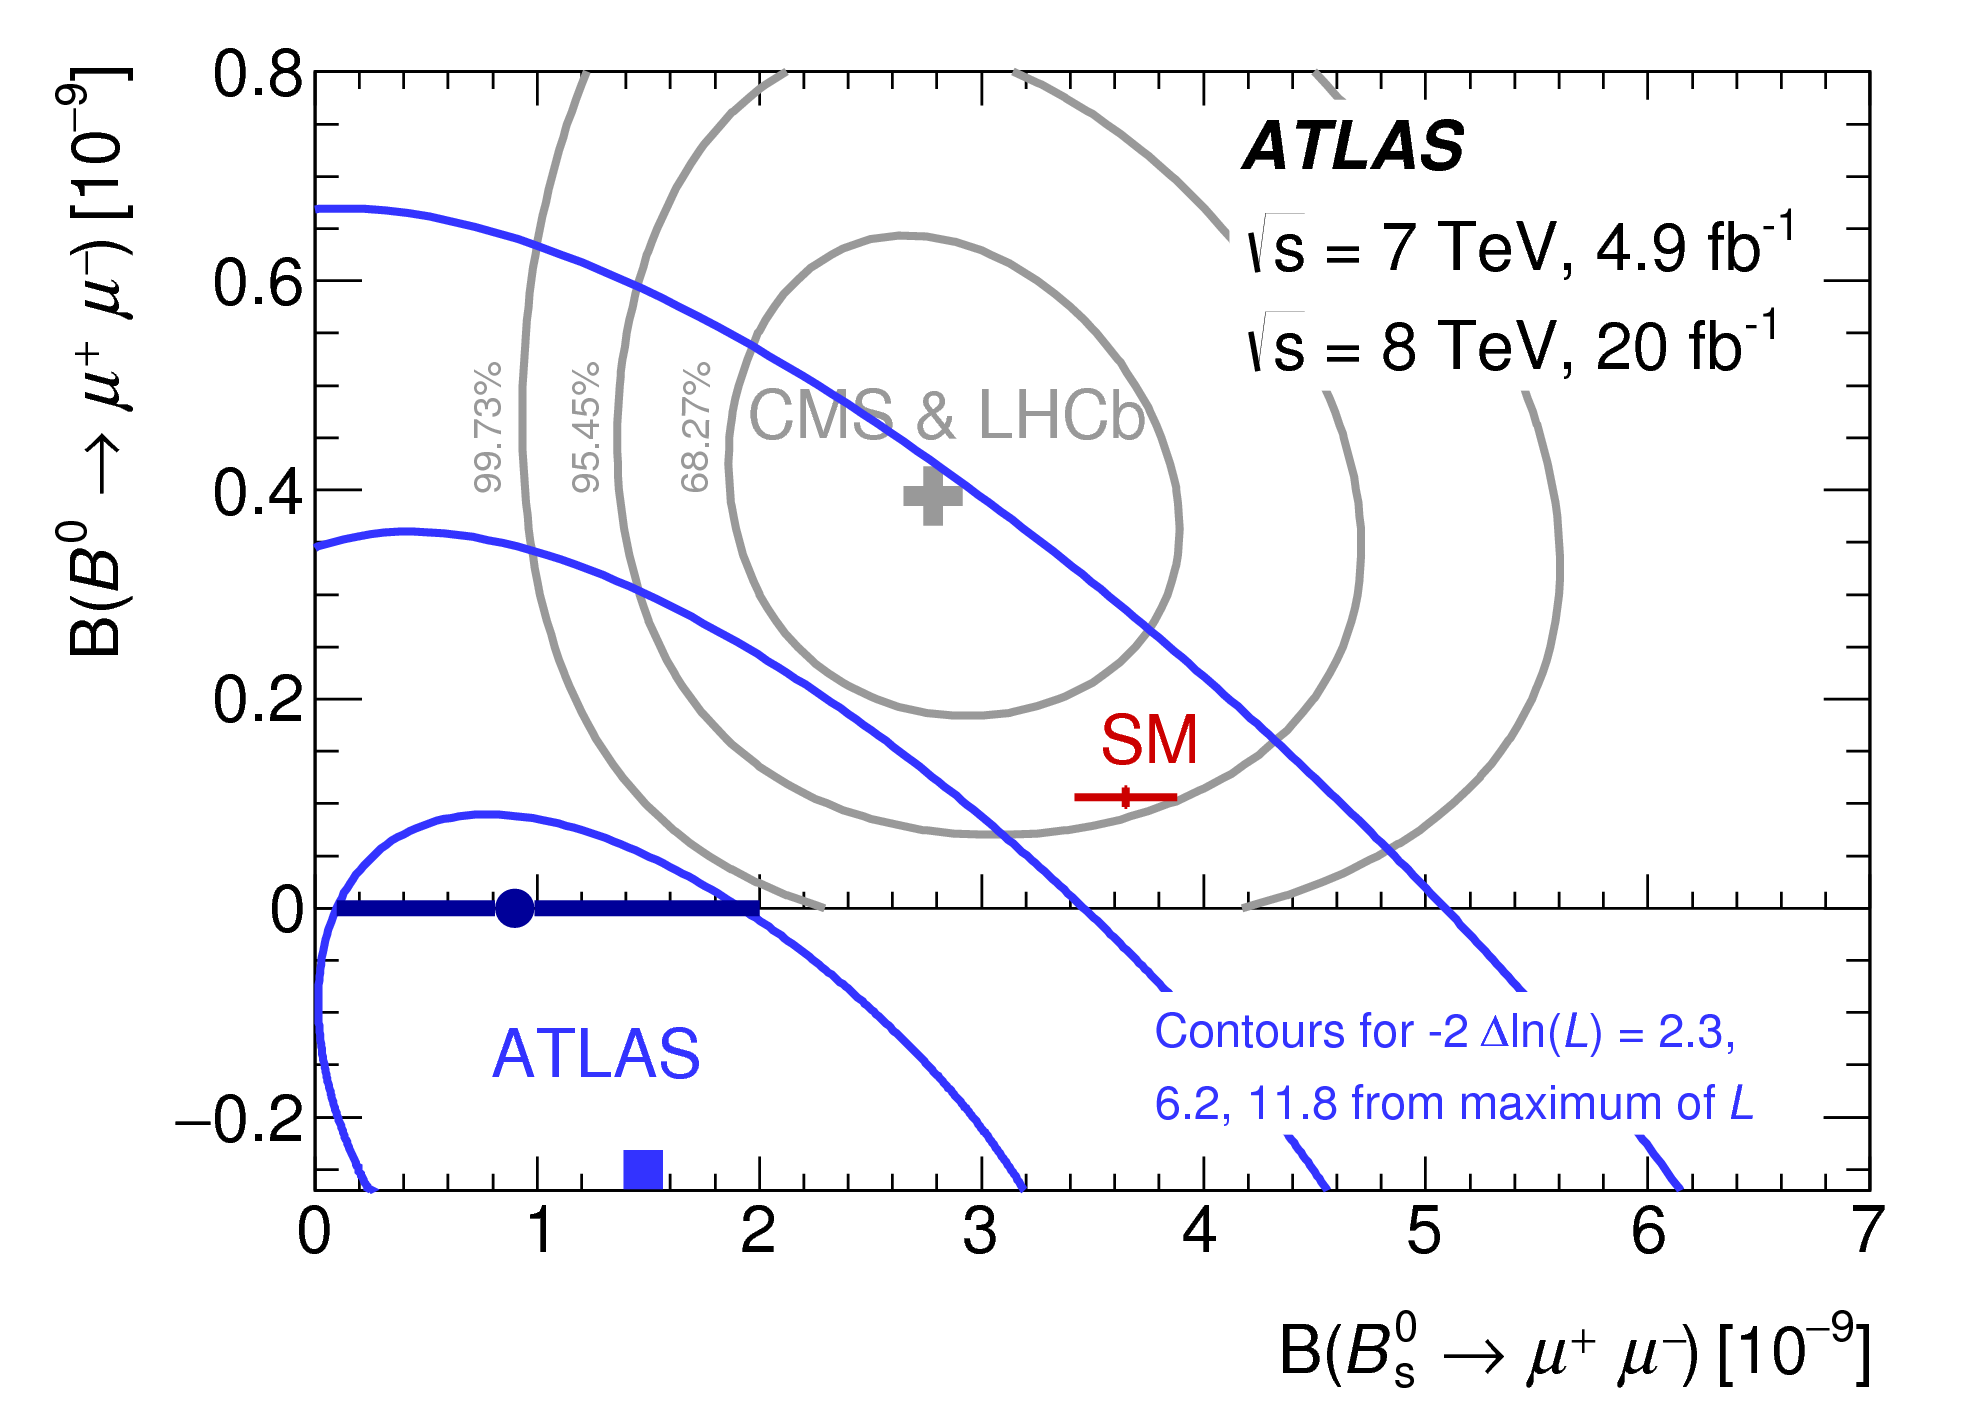
\includegraphics[width=0.6\textwidth]{fig_09.png}
    \caption
        {Contours in the plane  BR($B^0_s \to \mu \mu$), BR($B^0_d \to \mu \mu$) for intervals of
          $-2\, \Delta \ln(L)$ equal to $2.3$, $6.2$ and $11.8$ relative to the absolute maximum 
          of the likelihood (blue square), without imposing the constraint of non-negative branching fractions. 
          Also shown are the corresponding contours for the combined result of the CMS and LHCb 
          experiments, the SM prediction, and the maximum of the likelihood within the boundary of non-negative 
          branching fractions (blue dot), with the error bars covering the 68.3\% confidence range for BR($B^0_s \to \mu \mu$).}
        \label{fig:BsBd}
  \end{center}
\end{figure}
\section{Electroweak penguins decays}
Similarly to $B^0_{(s)} \to \mu \mu$ decays, also $b \to s l^+ l^-$ transitions are suppressed in the SM and then very sensible to New Physics processes. These decays are forbidden at the lowest perturbative order and proceed through loops involving electroweak penguin diagrams. Contrary to $B^0_{(s)} \to \mu \mu$ decays, the $b \to s l^+ l^-$ transitions do not have any helicity suppression. This means that possible NP contributions can modify not only the branching ratios of the decays, but also the angular distributions of the particles in the final state. Eventual contributions from NP processes can be parameterised into the SM lagrangian using the effective field theory approach. This approach allows to describe any NP contribution simply using higher dimension operators $O_i$ and the energy scale $\Lambda_{NP}$ where NP phenomena should appear. The total lagrangian $L$, which includes NP contributions, can then be written as:
\begin{equation}
L = L_{SM}+\sum_i c_i \frac{O_i}{\Lambda^2_{NP}}
\label{eq:wilson}
\end{equation}
where $L_{SM}$ represents the SM lagrangian and $c_i$ are complex coefficients (called Wilson coefficients) related to the strength of the interaction. In the SM all $c_i$ coefficients are zero. Any significant discrepancy would then be a hint of the presence of NP phenomena.\\
Several decay topologies involving mesons and baryons that contain $b$-quark belong to this category. One of the most interesting channels is $B_d \to K^{*0} \mu^+ \mu^-$, where only the $K^{*0} \to K^+ \pi^-$ decay mode is considered. The SM predicts a branching ratio of $\approx 4.5 \times 10^{-7}$, and the full kinematic of the decay can be described by three angles and the invariant mass squared $q^2$ of the two muons in the final state. The measurement of the three decay angles and of the differential decay rate as a function of $q^2$ allows to extract specific parameters called $P'_i$ (referred to in the following as optimised observables since they are independent, at the first order, from the form-factors involved in the calculation) which can be directly related to the Wilson coefficients $c_i$ introduced above. \\
The most complete analysis has been performed by LHCb~\cite{mumuK_LHCb}, The branching ratio and the three angles have been measured simultaneously and the full set of $P'_i$ parameters was extracted. A partial angular analysis has also been performed by the CMS collaboration~\cite{mumuK_CMS}. The analysis led to the extraction of the forward-backward asymmetry $A_{FB}$  measured in the di-muon system. $A_{FB}$ is another observable entering in the formula which describes the differential decay rate for this channel. Both ATLAS and CMS collaborations are preparing the full angular analysis on the full Run 1 dataset.  Figure~\ref{fig:mumuK} (left) shows the measurements of the $A_{FB}$ parameter as a function of $q^2$ performed by CMS experiment (compared with the SM prediction~\cite{ABSZ}), while Figure~\ref{fig:mumuK} (right) shows the measurement of one of the optimised observables (namely $P'_5$) as a function of $q^2$,  performed by the LHCb collaboration (compared with the values obtained by Belle collaboration~\cite{Belle} and the SM predictions). A discrepancy of the order of 2.8-3.0 $\sigma$, with respect to the SM predictions, has been reported by LHCb experiment for $q^2$ values between 4 and 8 ${\rm{GeV}}^2$.

Several other decay modes associated to the $b \to s \mu^+ \mu^-$ transition process have been considered by LHCb (such as $B^+ \to K^{+} \mu^+ \mu^-$, $B_s \to  \phi \mu^+ \mu^-$ and $\Lambda_b \to \Lambda \mu^+ \mu^-$). Each of these process is sensible to a different set of Wilson coefficients with respect to $B_d \to  K^{0*} \mu^+ \mu^-$ channel. The differential branching fractions as a function of $q^2$ have been measured for each channel and compared with the SM predictions. Some discrepancy with respect to the SM calculations, even if not significant, has been found also in some of these measurements.\\
\begin{figure}[!t]
  \begin{center}
  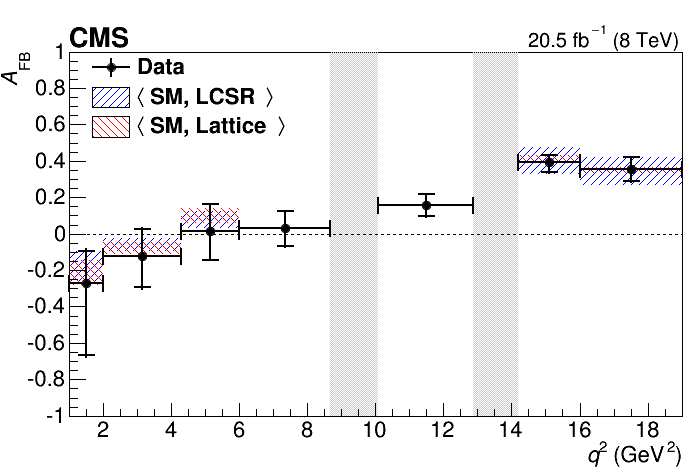
\includegraphics[width=0.48\textwidth]{AFB_CMS.png}
  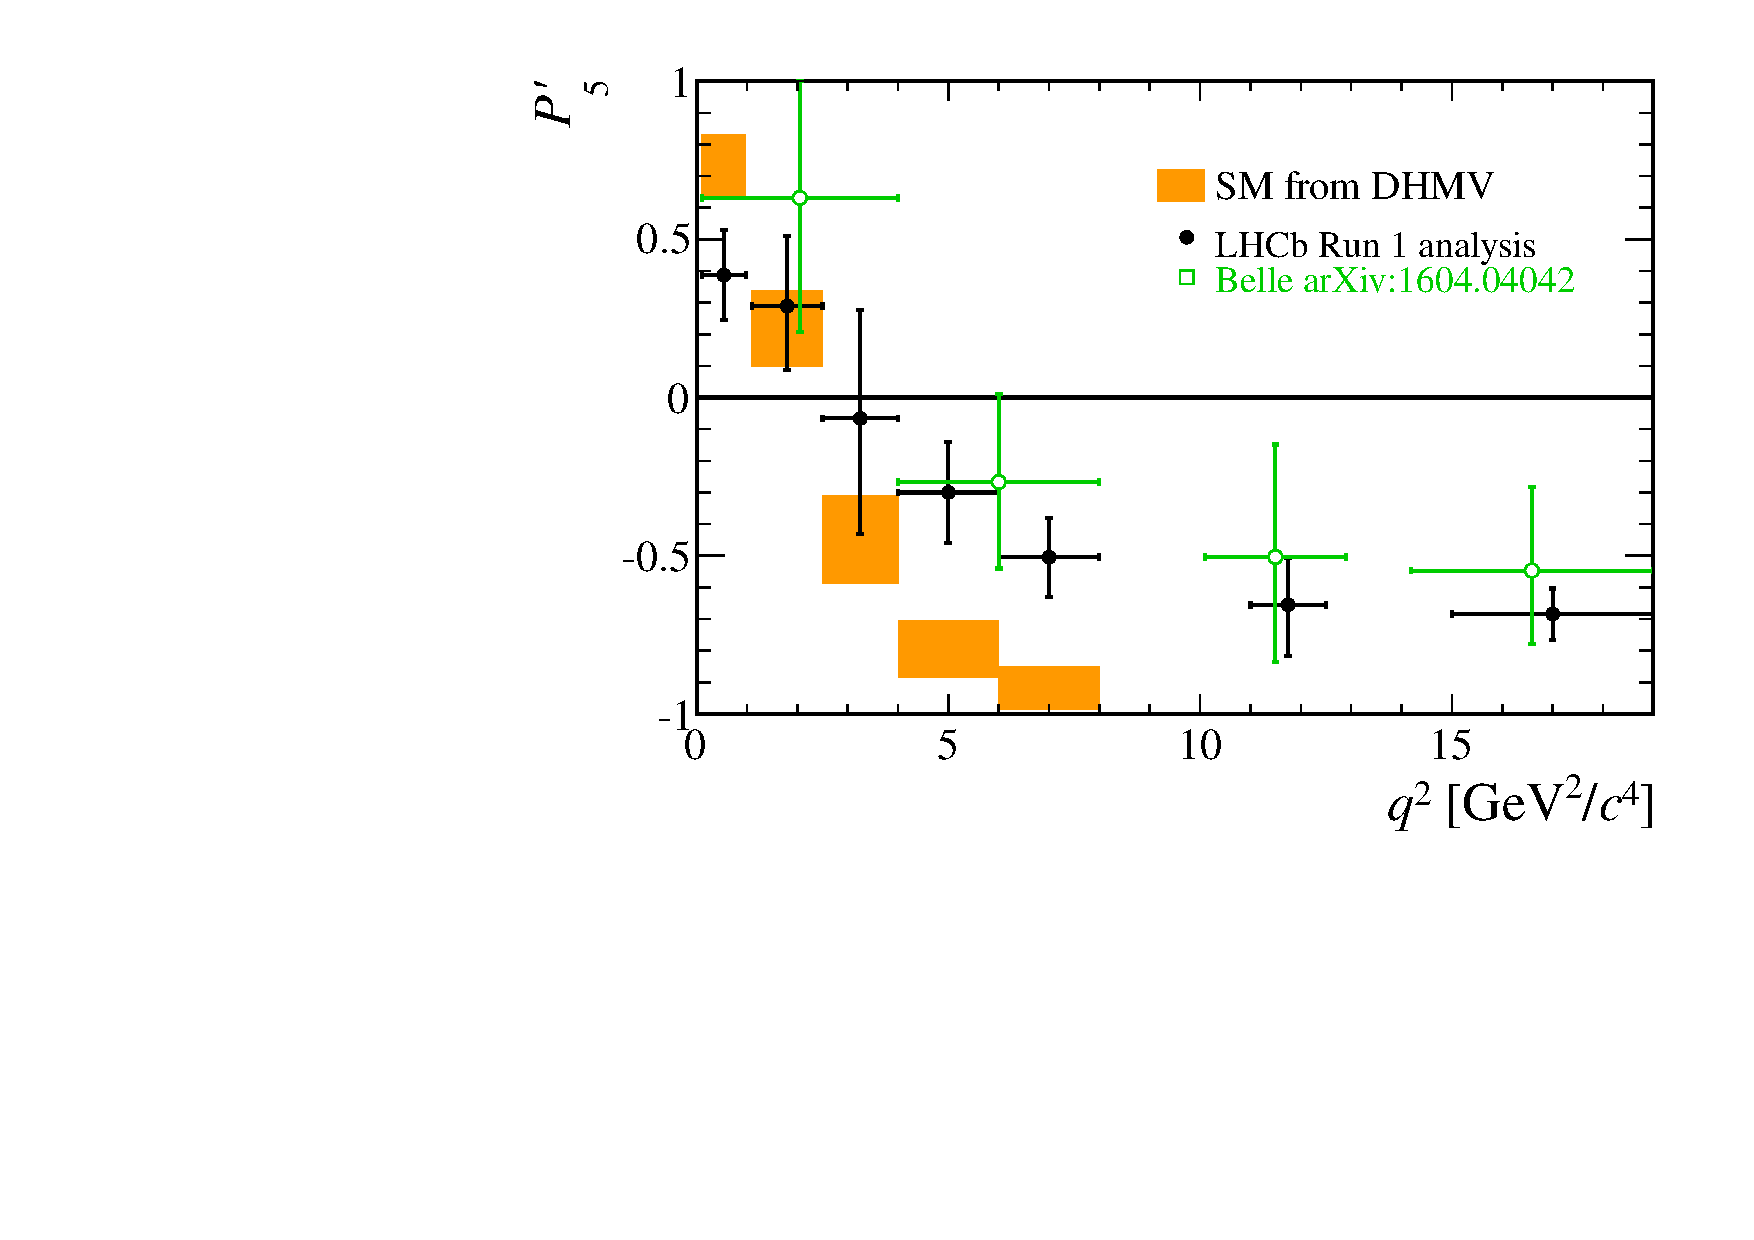
\includegraphics[width=0.48\textwidth]{P5p.pdf}
    \caption {(Left) $A_{FB}$ measurements as a function of $q^2$ as reported from several experiments. The SM predictions are taken from~\cite{ABSZ}. (Right) $P'_5$ distribution as a funciton of $q^2$ for the measurements performed by LHCb (black dots) and Belle (green) collaborations. The uncertainties include both statistical and systematic components.The SM predictions (yellow bands) are taken from~\cite{DHMV}. }
        \label{fig:mumuK}
  \end{center}
\end{figure}
The plan for Run 2 campaign of the three experiment in this domain is to systematically analyse several decay modes related to $b \to s \mu^+ \mu^-$  transitions in order to find any significant discrepancy of the optimised observables with respect to the SM predictions. LHCb experiment is also planning to perform the same set of measurements using electrons rather than muons in the final state. These measurements look instead very complicated for ATLAS and CMS experiments due to the different trigger menus and conditions available for the two experiments.

%\begin{thebibliography}{99}
%\bibitem{Bobeth} Bobeth C. et al., {\it{$B_{s,d} \to l^+ l^-$ in the Standard Model with Reduced Theoretical Uncertainty}}, Phys. Rev. Lett., {\bf{112}}, 101801, 2014.
%\bibitem{Nature} CMS and LHCb Collaborations, {\it{Observation of the rare $B^0_s\rightarrow\mu^+\mu^-$ decay from the combined analysis of CMS and LHCb data}}, Nature, {\bf{522}}, 2015.
%\bibitem{ATLAS} ATLAS Collaboration, {\it{Study of the rare decays of $B^0_s$ and $B^0$  into muon pairs from data collected during the LHC Run 1 with the ATLAS detector}}, arXiv:1604.04263 [hep-ex], 2016. {\it{Submitted to Eur.Phys. J. C}}.
%\bibitem{mumuK_LHCb} LHCb Collaboration, {\it{Angular analysis of the $B^0 \to K^{*0}  \mu^+ \mu^-$ decay using 3~${\rm{fb^{-1}}}$ of integrated luminosity}}, JHEP {\bf{02}} 104, 2016. 
%\bibitem{mumuK_CMS} CMS Collaboration, {\it{Angular analysis of the $B^0 \to K^{*0}  \mu^+ \mu^-$  decay from $pp$ collisions at $\sqrt{s} = 8$ TeV}}. Phys. Lett. B {\bf{753}} 424, 2016.
%\bibitem{Belle} Belle Collaboration, {\it{Angular analysis of $B^0 \to K^{*0}(892) \to l^+ l^-$}}, arXiv:[hep-ex] 1604.04042
%\bibitem{ABSZ} W. Altmannshofer and D.M. Straub, {\it{New physics in $b \to s$ transitions after LHC run 1}}, Eur. Phys. J. C {\bf{75}} (2015) 382 [arXiv:1411.3161].
%\bibitem{DHMV} S. Descotes-Genon, L. Hofer, J. Matias and J. Virto, {\it{On the impact of power corrections in the prediction of $B_d \to K^* \mu^+ \mu^-$ observables}}, JHEP {\bf{12}} (2014) 125 arXiv:1407.8526.
%\end{thebibliography}

%\end{document}

\section{Other rare decays}

While the core physics program of the LHCb experiment includes as a strong part the study of all 
$b$ and $c$- hadrons rare decays, owing to the very low transverse momenta involved, in some cases
ATLAS and CMS experiments can give only limited contributions. 

In this section we describe a set of studies which are important for their NP sensitivity 
but which results are almost exclusively from LHCb. 
We do not go in the detail of the measurements but give only a brief review of them.


\subsection{Lepton Flavour Violation}

The violation of lepton number (LNV) and lepton flavour conservation (LFV) are strictly prohibited
inside the SM, with the notable exception of neutrino oscillations, producing negligibly 
small effects in the charged sector. 
The discovery of a LNV or LFV decay of a known particle would be therefore a striking evidence 
of physics beyond the SM. 

A rich program of searches for LNV and LFV decays is undergoing at the LHC experiments. 
While the LHCb experiment can cover the full spectrum of beauty, charm and $\tau$ decays, 
the ATLAS and CMS experiments, given the low $p_T$ of the physical objects involved, do concentrate on specific decays which are easier to trigger. 

LHCb has set world best upper limits on $B^0_{(s)} \to e \mu$~\cite{Aaij:2013cby} 
and $D^0 \to e \mu$~\cite{Aaij:2015qmj} decays and has set a competitive
limit on $\tau \to \mu\mu\mu$ decays, contributing to improve the world combined limit \cite{Aaij:2014azz}. 
Also the ATLAS experiment has contributed recently on the same decay by looking for $\tau \to \mu\mu\mu$
where the $\tau$ comes from a $W$ boson leptonic decay~\cite{Aad:2016wce}; the sensitivity of this search is not yet 
competitive with LHCb and B-factories but proves the feasibility of such a delicate analysis in the high $p_T$ 
environment. 
Finally among the searches for LNV the most prominent is the LHCb search for prompt or long-living Majorana neutrinos 
in $B^+\to \pi^- \mu^+ \mu^+$ decays~\cite{Aaij:2012zr}.

Already exploiting Run I data, many other searches are in progress in the whole family of $B\to X e\mu$ decays and 
$B\to X \mu\tau$ decays where $X$ is a SM hadron. 

All the mentioned searches will be continued with Run II data aiming for NP or pushing further the limits on 
LFV and LNV couplings. 
During this period, Belle II experiment will start accumulating data and will compete strongly on the same channels. 
While channels with muons, being easy to trigger, are essentially limited by the collected luminosity, the others will
profit of the improved LHCb trigger in Run II and will stay as key measurement also for the Upgrade. 



\subsection{Radiative decays}

Rare radiative b-hadrons decays probing the FCNC $b\to s \gamma$ transition are complementary 
to $b\to s \ell \ell $ processes and are particularly sensitive to the $C_7$ Wilson coefficient. 

The LHCb core physics program includes also radiative $b$-hadron decays. 
In particular the LHCb experiment has obtained the first observation of the photon polarisation ~\cite{Aaij:2014wgo} in $b\to s \gamma$
transitions through the study of $B^+ \to K^+ \pi^+ \pi^-\gamma$ decays. 
Furtheremore  the ratio of branching fractions of the $B^0\to K^{\ast 0} \gamma$ and $B^0_s\to \phi \gamma$ decays has been measured
together with a search for direct CP asymmetry of the $B^0\to K^{\ast 0}\gamma$ decay~\cite{Aaij:2012ita}.
These measurements are only the start of a long program of measuremens of which a notable example will be 
the measurement of the effective lifetime of the $B^0_s \to \phi\gamma$ decay, which is strongly sensitive to new physics. 

The study of radiative $b$-hadron decays at ATLAS and CMS is difficult due to the low efficiency of reconstructing very low $p_T$ photons,
either directly or as $e^+e^-$ pairs. Therefore at present it is not foreseen a contribution of these two experiments in this field. 




\subsection{Rare charm decays}

Rare decays involving charm hadrons are fundamental probes of new physics: 
not only being complementary to $b$- and $s$-hadrons by probing the up sector, 
but also because FCNC are much more suppressed in charm due to the lack of a high mass down-type quark. 

A rich program of rare charm physics is brought forward by LHCb, ranging from FCNC to the already mentioned LFV decays. 
In particular the studies of $D^0\to \pi^+ \pi^- \mu^+\mu^-$~\cite{Aaij:2013uoa}, 
$D^0\to K^- \pi^+ \mu^+\mu^-$~\cite{Aaij:2015hva}, $D^+_{(s)}\to \pi^+ \mu^+\mu^-$~\cite{Aaij:2013sua} and $D^0\to \mu^+\mu^-$~\cite{Aaij:2013cza}
are putting strong bounds on NP scenarios, e.g. models with Leptoquarks~\cite{Bauer:2015knc}.
The $D^0 \to \mu^+ \mu^-$ decays has been studied also by the CMS experiment~\cite{Pedrini:2012vp}, however this was based on a loose trigger
configuration that could not be maintained.

The LHCb experiment will soon exploit Run II data and the study of rare charm decays will still be part of the core physics program
also in the upgrade phase. 
While ATLAS and CMS could explore the study of these decays exploiting events triggered independently by other particles, they are not expected to 
be competitive in the future on this domain. 
The Belle II experiment is expected to produce significant results in this field, but we do not discuss further this aspect here. 


% Please use the skeleton file you have received in the
% invitation-to-submit email, where your data are already
% filled in. Otherwise please make sure you insert your
% data according to the instructions in PoSauthmanual.pdf
%\documentclass{PoS}
%
%\title{Rare and semi-rare decays at ATLAS}
%
%\ShortTitle{Rare decays at ATLAS}
%
%\author{\speaker{Umberto De Sanctis}\thanks{on behalf of the ATLAS Collaboration}\\
%        University of Sussex\\
%        E-mail: \email{umberto.de.sanctis@cern.ch}}
%
%%\author{Another Author\\
%%        Affiliation\\
%%        E-mail: \email{...}}
%
%\abstract{}
%
%\FullConference{16th International Conference on B-Physics at Frontier Machines\\
%		2-6 May 2016\\
%		Marseille, France}
%
%\newcommand{\theInvRho}{\frac{\varepsilon_{\mu^+\mu^-}}{\varepsilon_{J/\psi K^{\pm}}}}
%\newcommand{\pt}{$p_{\rm{T}}$}
%\newcommand{\gev}{\rm{GeV}}
%
%\begin{document}
\section{Discussion}
The searches for rare and semi-rare decays of $B$ and $D$-mesons are central in the $B$-physics programme of all three experiments. As for all $B$-physics searches, the leading role is taken by the LHCb collaboration, whose detector was designed specifically for this type of physics. Nevertheless, ATLAS and CMS collaborations can be competitive in the searches for rare processes, that are basically limited by the size of the datasets to be analysed. In fact, both experiments will take advantage of the larger integrated luminosity they will be able to collect during Run 2 LHC campaign. Hence we envisage that, for some specific decay such as the $B_{(s)}^0 \to \mu \mu$ or those related to the $b \to s l^+ l^-$ transitions (see Section 2 and Section 3), the three experiments will be able to work together to combine their results to fully profit of the statistical power of the available datasets. A good step in this direction has been already made by CMS and LHCb collaborations in the combination of the $B_{(s)}^0 \to \mu \mu$ analyses and also by the creation of the LHCC Heavy-Flavour group. We hope that these steps will be the beginning of a fruitful collaboration among the LHC experiments.
%\end{document}


\begin{thebibliography}{99}
\bibitem{ATLAS} Armstrong, W. W. and others, 
{\it{ATLAS: Technical proposal for a general-purpose p p experiment at the Large Hadron Collider at CERN}},
CERN-LHCC-94-43 

\bibitem{CMS} CMS Collaboration, 
{\it{CMS, the Compact Muon Solenoid: technical proposal}},
LHC Tech. Proposal (1994) 
https://cds.cern.ch/record/290969

\bibitem{LHCb} LHCb Collaboration, 
{\it{LHCb : Technical Proposal}},
Tech. Proposal (1998) https://cds.cern.ch/record/622031

\bibitem{Bobeth} Bobeth C. et al., {\it{$B_{s,d} \to l^+ l^-$ in the Standard Model with Reduced Theoretical Uncertainty}}, Phys. Rev. Lett., {\bf{112}}, 101801, 2014.
\bibitem{Nature} CMS and LHCb Collaborations, {\it{Observation of the rare $B^0_s\rightarrow\mu^+\mu^-$ decay from the combined analysis of CMS and LHCb data}}, Nature, {\bf{522}}, 2015.
\bibitem{ATLAS_Bmumu} ATLAS Collaboration, {\it{Study of the rare decays of $B^0_s$ and $B^0$  into muon pairs from data collected during the LHC Run 1 with the ATLAS detector}}, arXiv:1604.04263 [hep-ex], 2016. {\it{Submitted to Eur.Phys. J. C}}.
\bibitem{mumuK_LHCb} LHCb Collaboration, {\it{Angular analysis of the $B^0 \to K^{*0}  \mu^+ \mu^-$ decay using 3~${\rm{fb^{-1}}}$ of integrated luminosity}}, JHEP {\bf{02}} 104, 2016. 
\bibitem{mumuK_CMS} CMS Collaboration, {\it{Angular analysis of the $B^0 \to K^{*0}  \mu^+ \mu^-$  decay from $pp$ collisions at $\sqrt{s} = 8$ TeV}}. Phys. Lett. B {\bf{753}} 424, 2016.
\bibitem{ABSZ} Bobeth C. et al., {\it{The Decay $B \to K l^+ l^-$ at Low Hadronic Recoil and Model-Independent $\Delta B = 1$ Constraints}}, JHEP {\bf{01}} (2012) 107 \newline
Bobeth C. at al. {\it{General analysis of $\bar{B} \to \bar{K}^{(*)} l^+ l^−$ decays at low recoil}} Phys. Rev. {\bf{D 87}} (2012) 034016
\bibitem{Belle} Belle Collaboration, {\it{Angular analysis of $B^0 \to K^{*0}(892) \to l^+ l^-$}}, arXiv:[hep-ex] 1604.04042
\bibitem{DHMV} S. Descotes-Genon, L. Hofer, J. Matias and J. Virto, {\it{On the impact of power corrections in the prediction of $B_d \to K^* \mu^+ \mu^-$ observables}}, JHEP {\bf{12}} (2014) 125 arXiv:1407.8526.

\bibitem{Aaij:2013cby} 
  R.~Aaij {\it et al.} [LHCb Collaboration],
  ``Search for the lepton-flavor violating decays $B^0_s \rightarrow e^{\pm}\mu^{\mp}$ and $B^0 \rightarrow e^{\pm} \mu^{\mp}$,''
  Phys.\ Rev.\ Lett.\  {\bf 111}, 141801 (2013)
  doi:10.1103/PhysRevLett.111.141801
  [arXiv:1307.4889 [hep-ex]].
  %%CITATION = doi:10.1103/PhysRevLett.111.141801;%%
  %23 citations counted in INSPIRE as of 25 Jun 2016

\bibitem{Aaij:2015qmj} 
  R.~Aaij {\it et al.} [LHCb Collaboration],
  ``Search for the lepton-flavour violating decay $D^0 \to e^\pm\mu^\mp$,''
  Phys.\ Lett.\ B {\bf 754}, 167 (2016)
  doi:10.1016/j.physletb.2016.01.029
  [arXiv:1512.00322 [hep-ex]].
  %%CITATION = doi:10.1016/j.physletb.2016.01.029;%%
  %3 citations counted in INSPIRE as of 25 Jun 2016

%\cite{Aaij:2014azz}
\bibitem{Aaij:2014azz} 
  R.~Aaij {\it et al.} [LHCb Collaboration],
  ``Search for the lepton flavour violating decay τ$^{−}$ → μ$^{−}$ μ$^{+}$ μ$^{−}$,''
  JHEP {\bf 1502}, 121 (2015)
  doi:10.1007/JHEP02(2015)121
  [arXiv:1409.8548 [hep-ex]].
  %%CITATION = doi:10.1007/JHEP02(2015)121;%%
  %27 citations counted in INSPIRE as of 25 Jun 2016

%%\cite{Aaij:2011ex}
%\bibitem{Aaij:2011ex} 
%  R.~Aaij {\it et al.} [LHCb Collaboration],
%  ``Search for the lepton number violating decays $B^{+}\to \pi^- \mu^+ \mu^+$ and $B^{+}\to K^- \mu^+ \mu^+$,''
%  Phys.\ Rev.\ Lett.\  {\bf 108}, 101601 (2012)
%  doi:10.1103/PhysRevLett.108.101601
%  [arXiv:1110.0730 [hep-ex]].
%  %%CITATION = doi:10.1103/PhysRevLett.108.101601;%%
%  %39 citations counted in INSPIRE as of 25 Jun 2016

\bibitem{Aad:2016wce} 
  G.~Aad {\it et al.} [ATLAS Collaboration],
  ``Probing lepton flavour violation via neutrinoless $\tau \longrightarrow 3\mu$ decays with the ATLAS detector,''
  Eur.\ Phys.\ J.\ C {\bf 76}, no. 5, 232 (2016)
  doi:10.1140/epjc/s10052-016-4041-9
  [arXiv:1601.03567 [hep-ex]].
  %%CITATION = doi:10.1140/epjc/s10052-016-4041-9;%%

%\cite{Aaij:2012zr}
\bibitem{Aaij:2012zr} 
  R.~Aaij {\it et al.} [LHCb Collaboration],
  ``Searches for Majorana neutrinos in $B^-$ decays,''
  Phys.\ Rev.\ D {\bf 85}, 112004 (2012)
  doi:10.1103/PhysRevD.85.112004
  [arXiv:1201.5600 [hep-ex]].
  %%CITATION = doi:10.1103/PhysRevD.85.112004;%%
  %59 citations counted in INSPIRE as of 25 Jun 2016

\bibitem{Aaij:2014wgo} 
  R.~Aaij {\it et al.} [LHCb Collaboration],
  %``Observation of Photon Polarization in the b→sγ Transition,''
  Phys.\ Rev.\ Lett.\  {\bf 112}, no. 16, 161801 (2014)
  doi:10.1103/PhysRevLett.112.161801
  [arXiv:1402.6852 [hep-ex]].
  %%CITATION = doi:10.1103/PhysRevLett.112.161801;%%
  %30 citations counted in INSPIRE as of 26 Jun 2016

\bibitem{Aaij:2012ita} 
  R.~Aaij {\it et al.} [LHCb Collaboration],
  %``Measurement of the ratio of branching fractions $BR(B_0 \to K^{\star 0} \gamma)/BR(B_{s0} \to \phi \gamma)$ and the direct CP asymmetry in $B_0 \to K^{\star 0} \gamma$,''
  Nucl.\ Phys.\ B {\bf 867}, 1 (2013)
  doi:10.1016/j.nuclphysb.2012.09.013
  [arXiv:1209.0313 [hep-ex]].
  %%CITATION = doi:10.1016/j.nuclphysb.2012.09.013;%%
  %35 citations counted in INSPIRE as of 26 Jun 2016

\bibitem{Aaij:2013uoa} 
  R.~Aaij {\it et al.} [LHCb Collaboration],
 ``Search for the decay $D_0 \to \pi^+ \pi^- \mu^+ \mu^-$,''
  Phys.\ Lett.\ B {\bf 728}, 234 (2014)
  doi:10.1016/j.physletb.2013.11.053
  [arXiv:1310.2535 [hep-ex]].
  %%CITATION = doi:10.1016/j.physletb.2013.11.053;%%
  %13 citations counted in INSPIRE as of 25 Jun 2016

\bibitem{Aaij:2015hva} 
  R.~Aaij {\it et al.} [LHCb Collaboration],
  %``First observation of the decay $D^{0}\rightarrow K^{-}\pi^{+}\mu^{+}\mu^{-}$ in the $\rho^{0}$-$\omega$ region of the dimuon mass spectrum,''
  Phys.\ Lett.\ B {\bf 757}, 558 (2016)
  doi:10.1016/j.physletb.2016.04.029
  [arXiv:1510.08367 [hep-ex]].
  %%CITATION = doi:10.1016/j.physletb.2016.04.029;%%


\bibitem{Aaij:2013sua} 
  R.~Aaij {\it et al.} [LHCb Collaboration],
  %``Search for $D^+_s \to \pi^+ \mu^+ \mu^-$ and $D^+_s \to \pi^- \mu^+ \mu^+$ decays,''
  Phys.\ Lett.\ B {\bf 724}, 203 (2013)
  doi:10.1016/j.physletb.2013.06.010
  [arXiv:1304.6365 [hep-ex]].
  %%CITATION = doi:10.1016/j.physletb.2013.06.010;%%
  %41 citations counted in INSPIRE as of 25 Jun 2016

\bibitem{Aaij:2013cza} 
  R.~Aaij {\it et al.} [LHCb Collaboration],
  %``Search for the rare decay $D^0 \to \mu^+ \mu^-$,''
  Phys.\ Lett.\ B {\bf 725}, 15 (2013)
  doi:10.1016/j.physletb.2013.06.037
  [arXiv:1305.5059 [hep-ex]].
  %%CITATION = doi:10.1016/j.physletb.2013.06.037;%%
 
\bibitem{Bauer:2015knc} 
  M.~Bauer and M.~Neubert,
  %``Minimal Leptoquark Explanation for the R$_{D^{(*)}}$ , R$_K$ , and $(g-2)_g$ Anomalies,''
  Phys.\ Rev.\ Lett.\  {\bf 116}, no. 14, 141802 (2016)
  doi:10.1103/PhysRevLett.116.141802
  [arXiv:1511.01900 [hep-ph]].

 \bibitem{Pedrini:2012vp} 
  D.~Pedrini [CMS Collaboration],
  %``Search for the flavour-changing neutral current decay $D^0 \to \mu^+\mu^-$ in $pp$ collisions at $\sqrt{s} = 7$ TeV with CMS,''
  arXiv:1208.5908 [hep-ex].
  %%CITATION = ARXIV:1208.5908;%%

\end{thebibliography}


\end{document}
